\appendix
\titleformat{\chapter}[frame]
  {\huge\normalfont\sc} 
  {\filright\footnotesize\enspace ANNEXE \thechapter\enspace}  {8pt}
  {\filcenter} 
\addcontentsline{toc}{chapter}{Annexes}
\renewcommand{\thefigure}{A\arabic{figure}}
\setcounter{figure}{0}

\chapter*{Annexes}

\renewcommand{\figurename}{Annexe}
\begin{figure}[h]
  \begin{adjustbox}
  {
  addcode=
  	{\begin{minipage}{\width}}
  		{\caption{Illustration des types de mutations}
         \label{fig:somatique}
    \end{minipage}},
  rotate=90,
  center
  }
    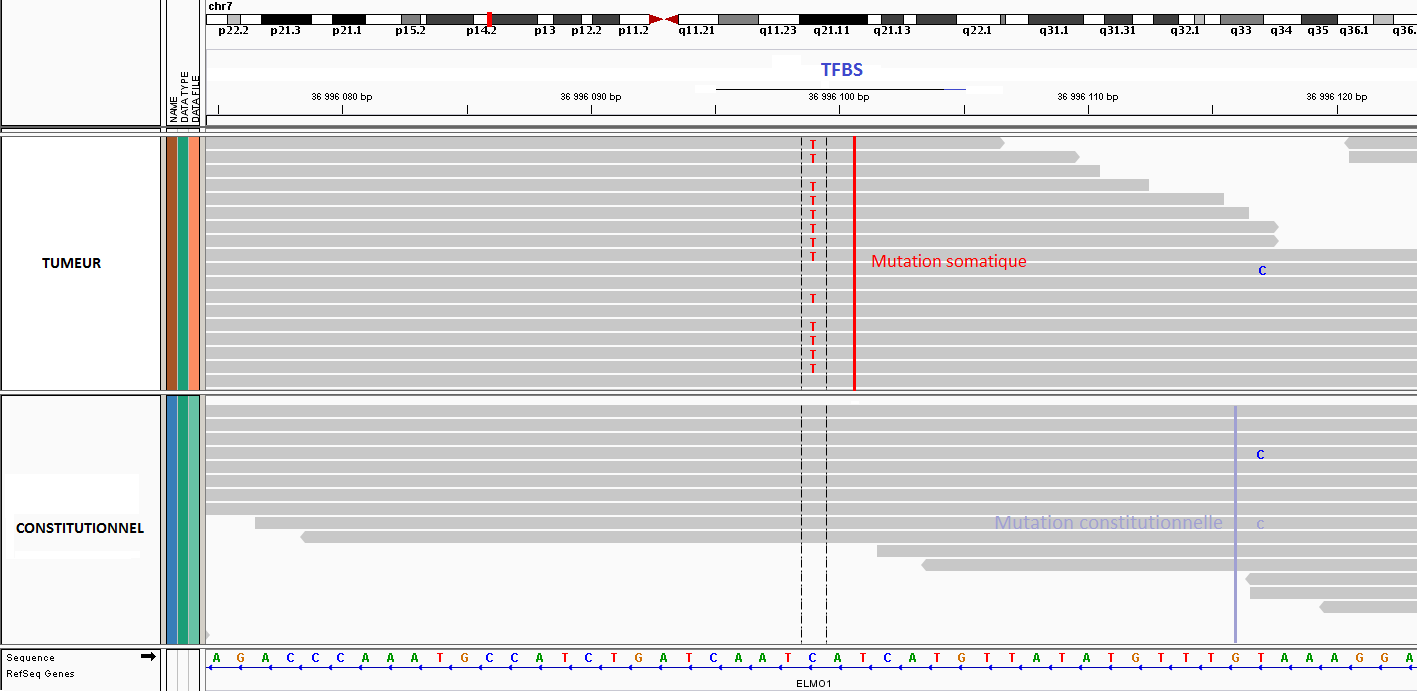
\includegraphics[height=15cm,width=21cm]{Figures/mutation.png}
  \end{adjustbox}
\end{figure}

